\documentclass[11pt]{article}
\usepackage[letterpaper,margin=0.7in]{geometry}
\usepackage{amsmath,booktabs,graphicx,microtype}
\usepackage[hidelinks]{hyperref}
\setlength{\parindent}{0pt}
\setlength{\parskip}{5pt}
\pagestyle{plain}
\begin{document}
\begin{center}
{\Large CS489 A3}\\[3pt]
\end{center}
\vspace{-8pt}
\section*{Setup and development results}

Each sentence was tokenized with its
original casing, special tokens and right padding, without truncation. For each
gold span, I averaged all of its WordPieces from the full-sentence hidden states,
excluding special tokens and padding. Layer 0 is the embedding-module output.

Each layer and seed used a fresh $768\to1024\to26$ MLP with biases and ReLU,
trained for 10 epochs using cross-entropy, Adam, learning rate $0.001$,
$\beta=(0.9,0.999)$, $\epsilon=10^{-8}$, weight decay $0$, and batch size 256.
I reset the random states and training shuffle for seeds 0--4, evaluated the full
development set after each epoch, and selected the highest accuracy, retaining
the earliest epoch on ties. Every best checkpoint was reloaded for final scoring.

\begin{center}
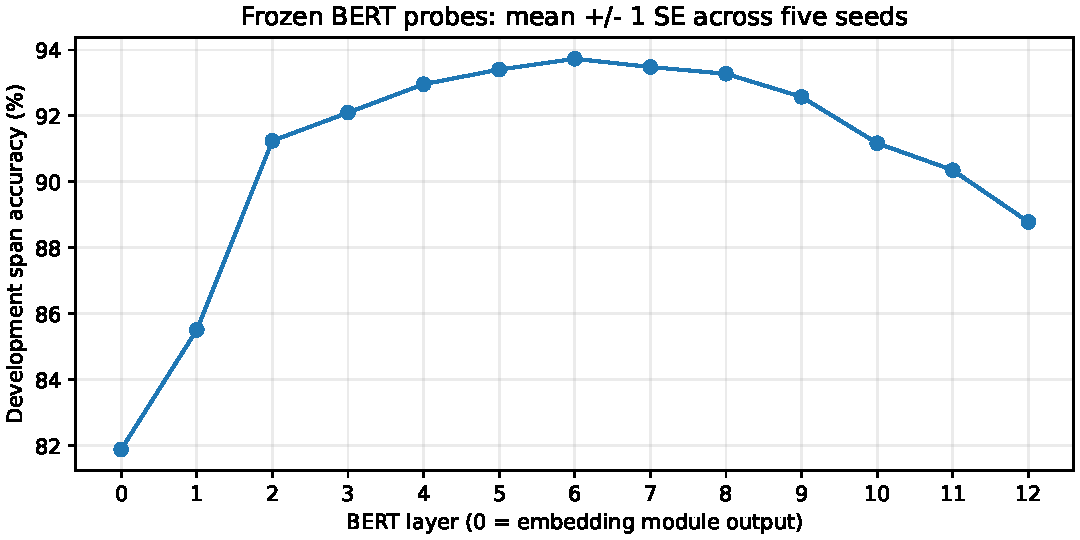
\includegraphics[width=0.94\linewidth]{layer_accuracy.pdf}\\[-2pt]
{\small Development performance of selected checkpoints: five-seed mean
$\pm$ one standard error.}
\end{center}
\vspace{-9pt}
\begin{center}
\small
\setlength{\tabcolsep}{9pt}
\begin{tabular}{rrr@{\hspace{22pt}}rrr}
\toprule
Layer & Accuracy (\%) & SE & Layer & Accuracy (\%) & SE\\
\midrule
0 & 81.883 & 0.042 & 7 & 93.479 & 0.034\\
1 & 85.509 & 0.029 & 8 & 93.274 & 0.055\\
2 & 91.241 & 0.057 & 9 & 92.574 & 0.042\\
3 & 92.096 & 0.060 & 10 & 91.168 & 0.078\\
4 & 92.958 & 0.042 & 11 & 90.351 & 0.037\\
5 & 93.402 & 0.034 & 12 & 88.781 & 0.017\\
\textbf{6} & \textbf{93.728} & \textbf{0.042} & & &\\
\bottomrule
\end{tabular}
\end{center}
\vspace{-7pt}


\newpage
\section*{Analysis}
\textbf{Q1}
Layer 6 has the highest mean development accuracy, 93.728\%. Early
representations improve substantially: layer 0 reaches 81.883\%, layer 1
85.509\%, and layer 3 92.096\%. Middle layers 4--8 all exceed 92.95\%, peaking
at layer 6. Accuracy then declines through the late layers: 92.574\% at layer 9,
90.351\% at layer 11, and 88.781\% at layer 12. The best layer exceeds the
embedding output by 11.845 pp and the final layer by 4.947 pp. Thus, the final
layer does not provide the best input to this fixed constituent-label probe.

\textbf{Q2}
The main differences between layers are much larger than the seed-to-seed
variation shown by the error bars. Layer 6 exceeds layers 0 and 12 by
11.845 and 4.947 pp, respectively, while the standard errors
across all layers range from only 0.017 to 0.078 pp.
Even the 0.249-point difference between layers 6 and 7 is much larger than
their standard errors of 0.042 and 0.034 points. In contrast, layers 5 and 7
differ by just 0.078 points, with standard errors of about 0.034 points each,
so this smaller difference is less clear relative to the variation across seeds. This particularly example shows small differences among nearby layers should be interpreted more cautiously.

\textbf{Q3}
With the same pooling, labels, probe and training budget, middle-layer features
make constituent labels easier for this MLP to recover. Above-embedding
performance is consistent with contextual representations adding useful
information. However, layer 0 already contains lexical, position and token-type
information, and its score shows that contextual blocks are not the only source
of predictive cues. The experiment measures what a supervised external
classifier can decode. It does not establish that BERT explicitly represents
parse trees, that its own predictions use these labels, or that the observed
information is causally necessary. Late-layer decline may reflect
representational changes that suit other objectives. It does not prove syntax
has disappeared.

\textbf{Q4}
Gold boundaries remove the need to discover constituents, so this is label
classification given spans, not full parsing. Annotation errors or inconsistent
analyses can limit accuracy and teach annotation-specific patterns. Overall
span accuracy weights frequent labels heavily and may hide weak performance on
rare classes. Mean pooling discards within-span order and boundary structure,
and weights words with more WordPieces more heavily. Full-sentence context
can supply label cues outside the span. Finally, a nonlinear 1,024-unit probe
can learn substantial task-specific mappings. Success does not imply the
labels are directly available to BERT, while failure under this fixed probe and
budget does not show that no other decoder could recover them.

\section*{Training Settings}
The experiment ran on a Google Colab Tesla T4 with Python 3.12. The logged preparation, training and final-evaluation time was
5,017 seconds, including 490 seconds for
feature preparation and 4,514 seconds for training and
per-run checkpoint checks. Setup and final plotting are outside this timer.

\section*{}
\textbf{AI Declaration:} Used ChatGPT for writing improvement and Codex for training script debugging and learning purposes.



\end{document}
